\subsection{Root finding}

Following ref. \cite{assignment}, the eigenvalues of the analytic solutions are given by the roots of the function $f(\lambda)$, shown in \cref{fig:f}. 
\begin{figure}
	\centering
	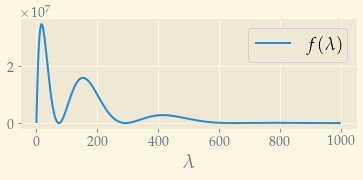
\includegraphics[width=\linewidth]{img/f}
	\caption{The analytic expression for finding the eigenvalues. }
	\label{fig:f}
\end{figure}
This is in good agreement with the computed eigenvalues. By using SciPy's \cite{2020SciPy-NMeth} optimized root-finding algorithm with the computed eigenvalues as the initial guess, we find three distinct eigenvalues below $\nu_0 = 10^3$.
Using the implementation of the root finder, the roots of $f(\lambda)$ is found more precicely, and the first couple of roots are shown in \cref{tab:roots}. 
\begin{table}
	\centering
\begin{tabular}{|c|c|}
	\hline
Computed $\bar\lambda$ & Roots of $f(\lambda) $\\
	\hline 
	73.49662578 & 73.93560016 \\ 

	73.49861656 &  \\ 

	291.77230762 & 293.49231502 \\ 
 
	291.79660664 &  \\ 
 
	644.62162712 & 648.26437316 \\ 

	645.10279446 &  \\
	\hline
\end{tabular}
	\caption{A comparison of computed eigenvalues and computed roots of the analytic expression for $f(\lambda)$. The units are given by \cref{eq:energy_conversion}. }
	\label{tab:roots}
\end{table}
Investigating the roots of $f(\lambda)$ for different values of $\nu_0$, we find that the value of $\nu_0$ that separates having one and no states with $\lambda < \nu_0$ is for 
\begin{equation} 
\nu_0 = 22.10526(3).
\end{equation}